\section{Technischer Regelkreis}
\subsection{Definitionen \formelbuch{14}}

\begin{description}[leftmargin=2.5cm]
 \item[System]	Eine Anordnung von Gebilden, welches von der Umwelt abgegrenzt ist, aber
								mit ihr über Inputs/Outputs in einer Beziehung stehen.
 \item[Prozess] Die Gesamtheit der zusammenwirkenden Vorgänge in einem System,
        		durch die Materie, Energie, Informationen umgeformt, transportiert und
        		gespeichert wird. \\
        		\begin{tabular}{lp{12cm}}
        		\textbf{ohne Ausgleich:} & Die Ausgangsgrösse ist für $t \rightarrow \infty$ nicht begrenzt \\
        		\textbf{mit Ausgleich:} & Die Ausgangsgrösse ist für $t \rightarrow \infty$ begrenzt. Ein Prozess wo sich selber ausgleicht wird oft mit einem $PT_1$-Glied modelliert.
        		\end{tabular}
 \item[Modell]	Ein Modell ist eine Abbildung eines Systems in ein anderes begriffliches oder
								gegenständliches System, dass den Prozess bezüglich ausgewählter Fragestellung
								hinreichend genau beschreibt.
 \item[SISO] Single Input - Single Output
 \item[MIMO] Multi Input - Multi Output
 \item[Steuerung]	Bei einer Steuerung wird der Energiestrom über mindestens einen Verstärker (Stelleinrichtung)
									beeinflusst, so dass die Prozessaufgabe erfüllt wird, wobei die Steuerinformation
									von Glied zu Glied läuft (Steuerkette) \newline
									-ohne Rückkopplung \newline
									- kann bei \textbf{stabiler} Strecke \textbf{nicht instabil} werden \newline
									- open loop\\
\begin{minipage}{8cm}
 \item[Regelung] mit Rückkopplung (wirkt als Gegenkopplung) \newline
 				 - immer ein Vergleichsglied zwischen Führungsgrösse (Sollwert) und
 				 Regelgrösse (Istwert) \newline
 				 - kann auf veränderte Störgrössen reagieren \newline
 				 - kann bei \textbf{stabiler} Strecke \textbf{instabil} werden. \newline
				 - closed loop
\end{minipage}
\begin{minipage}{8cm}
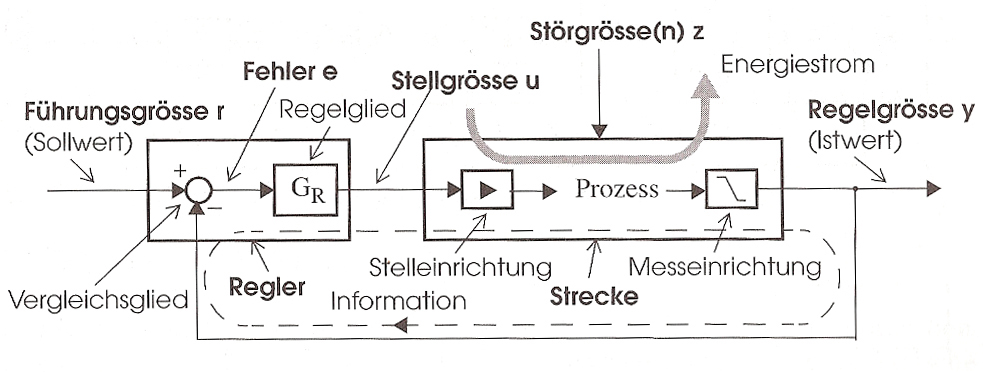
\includegraphics[width=8cm]{./bilder/Grundregelkreis_klein.jpg}
\end{minipage}				
				
\end{description}

	\begin{tabular}{|p{2.7cm}|p{5.4cm}|l|}
    	\hline
    	{\bf Begriff deutsch}		&{\bf Begriff englisch}	&{\bf Ergänzende
    	Erklärung} \formelbuch{20}\\
		\hline
		Regelung			& closed loop control ; control loop & Regelkreis\\
		\hline
		Regelstreck			& plant controlled system	&Der aufgabengemäss zu beeinflussende
    	Teil des Systems\\
    	\hline
    	Regler				& controller			&Bestehent aus Vergleichsglied und Regelglied\\
    	\hline
    	Regeleinrichtung	& controlling means&\\
    	\hline
    	Reglesignalkreis	& control circuit&\\
    	\hline
    	Vergleichsglied		& comparing element	&Bildet den Fehler (Differenz)
    											e=r-y\\
    	\hline
    	Regelglied			&controller;
    						controlling element	&Berechnet aus dem Fehler die Stellgrösse u\\
    	\hline
    	Stelleinrichtung
    	Verstärker			&actuator;
					    	power amplifier;
    						servo amplifier		&Funktionseinheit, die den Energie- oder Massenstrom
    											lenkt\\
    	\hline
    	Messeinrichtung
    	Messumformer		&measuring unit;
    						transmitter&\\
    	\hline
    	Regelgrösse y		&controlled variable;
    						desiered value& auch c oder x (DIN)\\
    	\hline
    	Führungsgrösse r	&reference variable;
    						set value& w (DIN)\\
    	\hline
    	Störgrösse z Last	&disturbance variable;
    						load& auch d\\
    	\hline
    	Stellgrösse u		&manipulatetd (correcting)
    						variable& y (DIN)\\
    	\hline
    	Regeldifferenz e	&deviation ; error variable		& Fehler: $e=r-y \quad \quad x_d=w-x$ (DIN) \\
    	\hline
    	Rückkopplung		&feedback			&Rückführung\\
    	\hline

	\end{tabular}\\

		
		%\begin{sidewaystable}
		\subsection{Klassifizierung technischer Systeme}
		\begin{tabular}{|l|l|p{6cm}|p{6cm}|}
        	\hline
        	
        	einfach &
        	schwierig &
        	Bemerkung &
        	Bedeutung des \textbf{ersten} Begriffs\\
        	\hline
        	
        	statisch &
        	\textcolor{red}{\underline{dynamisch}} &
        	&
        	Beschreiben nur den Gleichgewichtszustand (Vorgeschichte nicht
        	berücksichtigt)\\
        	\hline
        	
        	\textcolor{red}{\underline{linear}}	&
        	nichtlinear &
        	Ausnahmen: 2-, 3-Pt.Regler Simulation &
        	Assoziativ und Kommutativgesetz berücksichtigt \newline (x=X, 2x=2X;
        	y=Y, x+y=X+Y)\\
        	\hline
        	
        	\textcolor{red}{\underline{zeitinvariant}} &
        	zeitvariant &
        	&
        	unabhängig von zeitlicher Verschiebung \\
        	\hline
        	
        	\textcolor{red}{\underline{Zeitkontinuierlich}} &
        	zeitdiskret &
        	&
        	Signal hat zu jedem Zeitpunkt einen Wert\\
        	$\dot{y}=\frac{ku-y}{T}$ &
        	$y_{k+1}=a y_k + b u_k$	&
        	&
        	\\
        	\hline
        	
        	\textcolor{red}{\underline{wertkontinuierlich}}&
        	wertdiskret&
        	&
        	Signal kann alle Werte eines Intervalles annehmen\\
        	\hline
        	
        	\textcolor{red}{\underline{kausal}}	&
        	akausal	&
        	&
        	Die Ausgangsgrösse hängt nicht von zukünftigen Ereignissen ab\\
        	\hline
        	
        	\textcolor{red}{\underline{konzentrierte}} &
        	verteilte &
        	zB.	Stromleitung: &
        	\\
        	\textcolor{red}{\underline{Parameter}} &
        	Parameter	&
        	ein R und ein C/ sehr viele RC-Glieder in Serie &
        	\\
        	\hline
        	
        	\textcolor{red}{\underline{deterministisch}}	&
        	stochastisch &
        	vorhersehbar/zufällig &
        	Das Zeitverhalten lässt sich aufgrund seiner Gleichungen
        	``reproduzieren"\\
        	\hline
        \end{tabular}\\
				\textcolor{red}{\underline{wird für Regler vorausgesetzt!}}
       % \end{sidewaystable}